\documentclass{article}
\usepackage[dblblindworkshop]{neurips_2026}
\workshoptitle{Sim2Science}
\usepackage{amsmath,amssymb,amsfonts}
\usepackage{booktabs}
\usepackage{graphicx}
\usepackage{microtype}
\usepackage{xcolor}
\usepackage{url}
\usepackage{multirow}
\usepackage{hyperref}

\title{From RANS Prediction to Hydrofoil Optimization:\\
A Benchmark of Neural Surrogates}

\author{Anonymous Author(s)}

\begin{document}
\maketitle

\begin{abstract}
We benchmark four neural surrogates for hydrofoil RANS prediction and design:
CNN-U-Net, a physics-regularized point network, a Fourier neural operator
(FNO), and DeepONet. The dataset contains 381 valid OpenFOAM cases. The 64-case
validation set consists of two NACA families that are absent from training.
The models predict flow fields, force coefficients, and pressure-based
cavitation risk. The physics-regularized network gives the best pressure result
($R^2=0.966$) and cavitation-risk F1 score (0.921). DeepONet gives the best lift
and drag results ($R^2=0.996$ and $0.988$). Inference is 917--1801 times faster
than OpenFOAM. We then place each model in the same shape optimizer and rerun
its best design in OpenFOAM. The validated lift-to-drag improvements range from
2.3\% to 79.7\%. The benchmark connects predictive accuracy and computational
cost to the quality of the design produced downstream.
\end{abstract}

\section{Introduction}
Computational fluid dynamics (CFD) supports hydrofoil analysis and design, but
repeated Reynolds-averaged Navier--Stokes (RANS) solves make parameter sweeps and
optimization expensive. Neural surrogates can reduce this repeated cost
\citep{brunton2020machine}. A useful design surrogate must do more than match an
average flow field. It must preserve pressure and forces, identify low-pressure
regions, and guide an optimizer toward a design that still performs well when
it is returned to CFD.

CNN-U-Nets learn local multiscale structure \cite{ronneberger2015unet}. Fourier
neural operators learn global spectral mappings \cite{li2021fno,kovachki2023neural}.
DeepONet combines parameter and coordinate representations \cite{lu2021deeponet},
while physics-informed models add differential-equation residuals
\cite{raissi2019pinn}. These architectures make different assumptions about the
flow map. Comparing them on one dataset reveals where each assumption helps.

Earlier airfoil surrogates used convolutional or hybrid networks to predict
steady flow fields from geometry and operating conditions
\cite{guo2016steady,bhatnagar2019aerodynamic,sekar2019airfoils,thuerey2020rans}.
Physics-informed neural operators combine PDE residuals with operator learning
\cite{li2024pino}. We instead hold the data and optimizer fixed and compare how
four model families perform from flow prediction through design selection.

We use 381 valid OpenFOAM simulations covering twelve NACA families, eight
angles of attack, and four Reynolds numbers. All models use the same targets
and unseen-geometry validation set. We compare flow and force accuracy,
cavitation-risk classification, runtime, and continuous shape optimization.
Each model-selected design is then rerun in OpenFOAM. This final test asks a
simple question: does the surrogate lead the optimizer to a better hydrofoil?

Our contributions are:
\begin{itemize}
    \item a four-model benchmark on an unseen-geometry validation set, covering
    flow fields, force coefficients, runtime, and cavitation-risk screening;
    \item a common hydrodynamic shape-optimization experiment; and
    \item an OpenFOAM rerun of every model's selected design.
\end{itemize}

We intentionally make a limited cavitation claim. The present labels measure pressure-threshold inception risk derived from single-phase RANS pressure. They do not model vapor fraction, cavity length, collapse, or shedding, which require multiphase simulations or experiments.

\section{Data and CFD Reference}
\subsection{Design space}
The dataset contains NACA 0006, 0008, 0010, 0012, 0015, 0018, 2412, 2415, 4412, 4415, 4418, and 4421 profiles generated from the standard four-digit parameterization \cite{abbott1959airfoils}. For each profile, we simulate angles of attack $\alpha\in\{-4,-2,0,2,4,6,8,10\}^{\circ}$ and Reynolds numbers $Re\in\{10^5,2\times10^5,5\times10^5,10^6\}$. The chord is 1~m, water density is 997~kg/m$^3$, and kinematic viscosity is $10^{-6}$~m$^2$/s, so the freestream speed is set by $U_\infty=Re\nu/c$. The far-field absolute pressure and vapor pressure are 101325 and 2300~Pa.

Each case is solved with OpenFOAM \texttt{simpleFoam} \cite{weller1998tensorial}, using steady incompressible RANS and the $k$--$\omega$ SST closure \cite{menter1994sst}. Angled freestream velocity is imposed at the inlet and far boundary. The solver runs for 300 iterations, and OpenFOAM's \texttt{forceCoeffs} provides total lift and drag references. Cell-centered fields are interpolated to a common $128\times64$ Cartesian grid over $x/c\in[-1,2]$ and $y/c\in[-0.75,0.75]$. Inputs include coordinates, operating parameters, three NACA geometry descriptors, a fluid mask, and signed distance to the profile.

An audit found no pressure fields duplicated across angle of attack and found force files for all 384 cases. Three cases (NACA 0006 at $10^\circ$, NACA 0008 at $-4^\circ$, and NACA 4412 at $0^\circ$) produced $|C_L|$ or $|C_D|>5$ and were excluded before splitting. This leaves 381 cases. The deterministic geometry split holds out all 64 cases from NACA 0015 and NACA 2412; the remaining 317 cases train the models. Holding out complete families prevents identical geometry from appearing at different operating conditions in both partitions.

\subsection{Targets and cavitation-risk definition}
The common output vector contains $U_x$, $U_y$, absolute pressure $p$, eddy viscosity, $k$, $\omega$, $C_p$, cavitation margin, $C_L$, and $C_D$. Grid fields use masked normalized mean-squared error, while the case-level force targets use normalized mean-squared error. OpenFOAM's kinematic gauge pressure $p_k$ is converted to absolute pressure as
\begin{equation}
 p=p_\infty+\rho p_k, \qquad C_p=\frac{p-p_\infty}{\tfrac{1}{2}\rho U_\infty^2}.
\end{equation}
For an ambient-pressure value $p_a$, the pressure-based inception margin is
\begin{equation}
 M(x,y;p_a)=p_a+C_p(x,y)\tfrac{1}{2}\rho U_\infty^2-p_v.
\end{equation}
A cell is labeled at risk when $M<0$. We evaluate this label at $p_a\in\{2500,3000,5000,10000,25000,101325\}$~Pa. This sweep creates a useful classification test from the predicted $C_p$ field without representing multiphase physics.

\section{Surrogates and Optimization}
\subsection{Model families}
The \textbf{CNN-U-Net} has three encoder/decoder levels, skip connections,
group normalization, GELU activations, and base width 16. The \textbf{FNO} has
width 32, four operator blocks, and 12 retained Fourier modes per direction
\cite{ronneberger2015unet,li2021fno}:
\begin{equation}
h_{l+1}=\sigma\!\left(W_lh_l+\mathcal{F}^{-1}(R_l\mathcal{F}(h_l))\right).
\end{equation}
The \textbf{DeepONet} uses three-layer, width-64 branch and trunk networks with
64 basis functions. Its output has the form
\begin{equation}
\widehat y_k(\mathbf{x};\boldsymbol{\mu})=
\mathbf{b}_k(\boldsymbol{\mu})^\top\mathbf{t}_k(\mathbf{x})/\sqrt{64}+c_k.
\end{equation}
following \cite{lu2021deeponet}.
The \textbf{physics-regularized point network} has three tanh layers of width
64 and uses 1,024 sampled points per case. Its supervised loss is augmented by
$10^{-4}$ times the continuity and first-order momentum residual loss
\cite{raissi2019pinn}. This is
a lightweight physics regularizer, not a data-free PINN or complete RANS
residual.

All models use AdamW with learning rate $2\times10^{-3}$, weight decay
$10^{-4}$, at most 120 epochs, patience 20, gradient clipping, and seed 7.
Normalization uses training cases only. The best checkpoint is selected by
validation loss. Model size ranges from 9,930 to 595,914 parameters
(Table~\ref{tab:performance}).

Although surface-pressure integration was implemented as a diagnostic, the coarse common grid did not reproduce absolute OpenFOAM forces reliably because it omits viscous traction and under-resolves the wall. Therefore, optimization uses dedicated $C_L$ and $C_D$ output heads trained on OpenFOAM's total force coefficients. This choice avoids presenting an invalid pressure-only force calculator as ground truth, but it also means force prediction is directly supervised.

\subsection{Common optimization protocol}
At $Re=5\times10^5$, every model optimizes the NACA variables $\theta=(m,p,t,\alpha)$ from NACA 0012, 2412, and 4415 starts. Bounds are $m\in[0,0.09]$, $p\in[0.1,0.9]$, $t\in[0.06,0.20]$, and $\alpha\in[-4,10]^{\circ}$. Nelder--Mead \cite{nelder1965simplex} runs for at most 40 iterations with identical tolerances. The objective is
\begin{equation}
J(\theta)=\frac{C_L}{|C_D|+10^{-6}}-10P_M-5f_M,
\end{equation}
where $P_M$ penalizes a predicted minimum cavitation margin below 5000~Pa and $f_M$ is the fraction of cells below that margin. At the nominal ambient pressure, all selected designs remain far above the threshold, so the cavitation penalty is inactive; the separate ambient-pressure sweep evaluates inception classification under reduced pressure. For each architecture, we select the highest-scoring design across starts and create a new mesh and OpenFOAM case without using surrogate predictions to initialize the solver.

\section{Results}
\subsection{Validation accuracy and computational cost}
Table~\ref{tab:performance} reports results on the 64-case validation set. The physics-regularized network is best for pressure and $C_p$, with pressure RMSE 6.78~Pa and $R^2=0.966$. DeepONet gives the best $U_x$, $U_y$, $C_L$, and $C_D$ coefficients. The grid operators are weaker in this low-data setting. FNO retains useful force trends, while CNN-U-Net predicts $C_p$ and forces better than absolute pressure or streamwise velocity.

\begin{table}[t]
\caption{Validation performance, model size, and cost. Force RMSE is computed case-wise against OpenFOAM total coefficients.}
\label{tab:performance}
\centering
\resizebox{\columnwidth}{!}{%
\begin{tabular}{lrrrrrr}
\toprule
Model & $p$ RMSE & $p$ $R^2$ & $C_L$ RMSE & $C_D$ RMSE & Params. & Speedup \\
\midrule
CNN-U-Net & 28.52 & 0.392 & 0.0991 & 0.00453 & 485,178 & 1,148$\times$ \\
Physics-reg. MLP & \textbf{6.78} & \textbf{0.966} & \textbf{0.0245} & 0.00204 & \textbf{9,930} & \textbf{1,801$\times$} \\
FNO & 22.73 & 0.614 & 0.1383 & 0.00957 & 595,914 & 1,028$\times$ \\
DeepONet & 8.55 & 0.945 & 0.0268 & \textbf{0.00184} & 100,746 & 917$\times$ \\
\bottomrule
\end{tabular}}
\end{table}

Measured training times are 868, 104, 547, and 54~s for CNN-U-Net, the physics-regularized network, FNO, and DeepONet, respectively. Median OpenFOAM execution time is 12.4~s per case, while pressure-field inference requires 0.0069--0.0135~s, yielding 917--1801$\times$ speedups. The benchmark used an 8-core Apple M2 Mac mini with 16~GB memory; PyTorch 2.13 ran on CPU and single-process OpenFOAM 9 ran in Docker. These numbers measure repeated local inference and exclude data generation and mesh construction.

Figure~\ref{fig:pressure} shows a representative validation case from the unseen NACA 0015 family. The
pointwise models reproduce the leading-edge pressure structure most closely;
CNN-U-Net smooths the extrema and FNO introduces spatial texture. The distinct
error color scales in the lower row are retained to expose each model's error
structure rather than visually equalizing models with very different ranges.

\begin{figure*}[t]
\centering
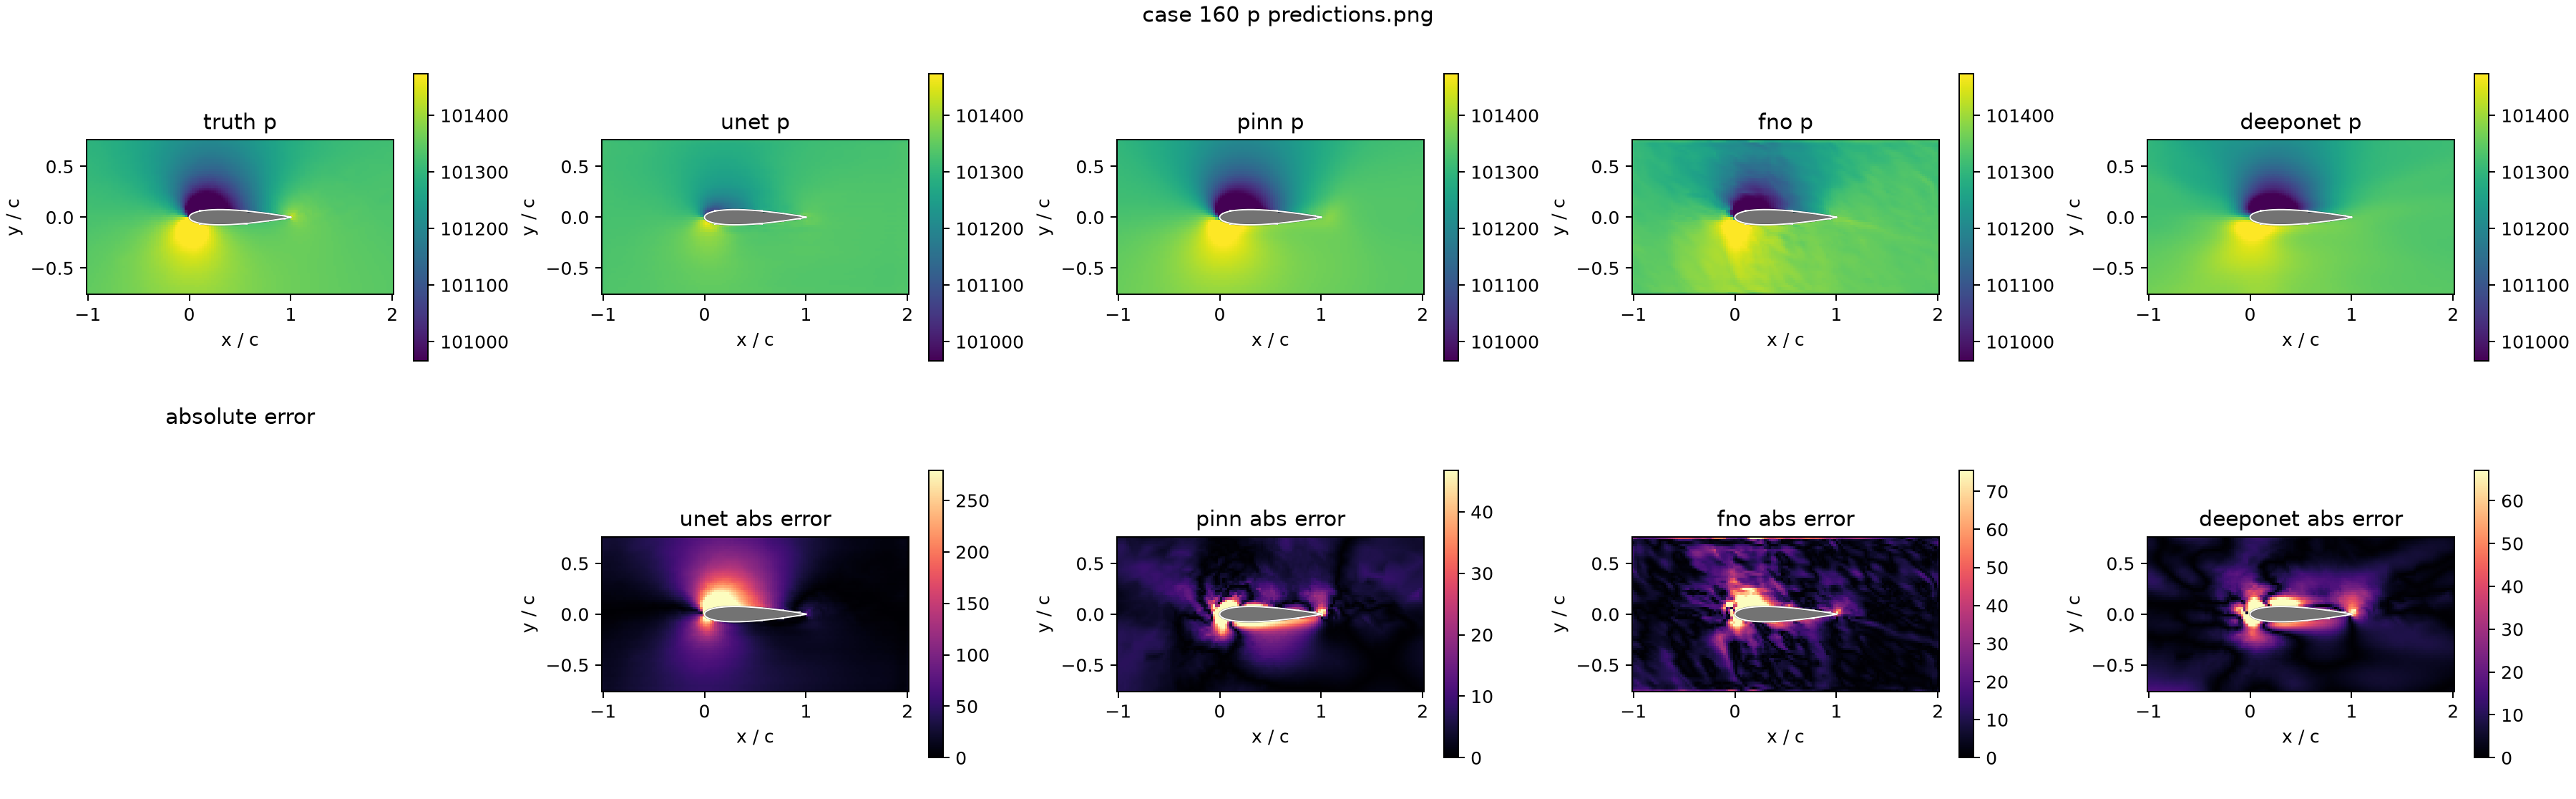
\includegraphics[width=0.82\textwidth]{figures/heldout_pressure.png}
\caption{Absolute-pressure prediction for a representative validation case from the NACA 0015
case (case 160), followed by per-model absolute error. All prediction panels
share the truth color scale; error panels use individually labeled scales.}
\label{fig:pressure}
\end{figure*}

\subsection{Cavitation-inception screening}
The pressure-threshold labels are highly imbalanced, so accuracy is not useful here. The physics-regularized network achieves precision 0.927, recall 0.916, and F1 0.921. DeepONet follows at F1 0.913. CNN-U-Net has the highest recall (0.958) but lower precision (0.796), while FNO obtains F1 0.771. Twenty-four validation case/ambient-pressure combinations contain at-risk cells. This measures pressure-based inception screening, not cavity dynamics. Multiphase labels are required to predict vapor fraction, cavity length, or shedding \cite{brennen1995cavitation}.

\subsection{CFD-revalidated optimization}
Table~\ref{tab:optimization} compares each model's predicted winner with a fresh OpenFOAM solve. All four winners improve upon their associated starting foil in CFD, but by very different amounts. The physics-regularized network selects a thin, strongly cambered profile whose validated $L/D=45.96$ is 79.7\% above the NACA 4415 baseline. DeepONet obtains a 57.8\% improvement and CNN-U-Net obtains 48.5\%. FNO predicts the lowest-performing winner; revalidation gives only a 2.3\% gain over its baseline.

\begin{table}[t]
\caption{Surrogate-selected winners and independent OpenFOAM revalidation. Improvement is relative to the corresponding start at the optimization condition.}
\label{tab:optimization}
\centering
\resizebox{\columnwidth}{!}{%
\begin{tabular}{lrrrrr}
\toprule
Model & Start & Pred. $L/D$ & CFD $L/D$ & Error & CFD gain \\
\midrule
CNN-U-Net & 2412 & 30.17 & 38.45 & $-21.5\%$ & 48.5\% \\
Physics-reg. MLP & 4415 & 43.62 & 45.96 & $-5.1\%$ & \textbf{79.7\%} \\
FNO & 4415 & 21.11 & 26.15 & $-19.3\%$ & 2.3\% \\
DeepONet & 2412 & 39.99 & 40.86 & $-2.1\%$ & 57.8\% \\
\bottomrule
\end{tabular}}
\end{table}

The optimization test sharpens the field benchmark in two ways. First, DeepONet gives the smallest winner-level $L/D$ discrepancy, consistent with its force accuracy, but the physics-regularized model finds the best validated design. Second, the FNO winner improves after CFD revalidation yet remains close to its baseline, showing that a conservative prediction error does not guarantee strong search guidance. Screening of five randomly perturbed profiles and an oval was also performed, but these geometries lie outside the NACA training manifold and are reported only as stress tests, not validated free-form design evidence.

\section{Scope and Next Steps}
The pointwise models lead in this low-data, fixed-grid experiment. This is not a
universal ranking. It is a controlled comparison in which every model sees the
same data, targets, split, and optimizer. Larger datasets or different loss
balancing may favor the grid operators.

Pressure, force, and optimization metrics answer different questions. DeepONet
is the best force model, but the physics-regularized network returns the best
CFD-validated design. This difference is the main reason to include optimization
in the benchmark instead of stopping at validation error.

The current study covers two-dimensional, steady, single-phase RANS and NACA
four-digit profiles. Three divergent cases are removed by a fixed quality rule,
and a symmetry audit finds a small lift bias. Force coefficients are directly
supervised because the common grid cannot resolve surface forces accurately.
One winner per model is rerun. Cavitation results cover inception risk, not vapor
transport or shedding. Repeated seeds, mesh sensitivity, multiphase labels, and
more CFD checks around each optimum are the clearest next steps.

\section{Conclusion}
Across four neural surrogates, the physics-regularized point network gives the
strongest joint pressure, inception-risk, speed, and validated-design result,
while DeepONet predicts forces most accurately. The 917--1801$\times$ speedups
make search practical, and the OpenFOAM reruns show how prediction differences
carry into design. The optimization experiment makes the comparison more useful
than a field-only ranking.

\section*{Artifact Availability}
Code, configurations, split definitions, trained checkpoints, per-case metrics, optimization traces, and OpenFOAM validation cases are organized in an auditable repository. An anonymized archival link will be added before submission.

\bibliographystyle{plainnat}
\bibliography{references}

\input{checklist}

\end{document}
